\chapter{Results}
\label{chap:findings}
This chapter presents the results of this thesis based on the two parts of the study. First, the results of the session with usability experts are presented. Second, the results of the session with CRM users are presented. Both of these sections consist of a description of the participants and an overview and analysis of the outcomes. Finally, a comparative analysis is conducted to investigate the commonalities and differences between the results of the first and second phases. Finally, a unified list of usability heuristics for web-based CRM systems is created.

\section{Phase One}
The first session was administered on June 28th, 2012, and took 2.5 hours. During the first segment, which lasted approximately one hour, participants were briefed and then rated existing heuristics presented to them in the group support system. After a break, the participants engaged in a group discussion during which they were asked to reword those heuristics which were identified to be in need of rewording to be more applicable to web-based CRM systems. Finally, the participants were asked to develop new heuristics specific to web-based CRM systems in a group discussion. The two discussions in the second part of the session took one hour.

\subsection{Participants}
Five usability experts participated in the first session. Table~\ref{tab:first_participants} gives an overview of the participants' experience relevant to this study. All participants had at least four years of experience evaluating, designing, or developing user interfaces, and at least 2.5 years of professional experience in the usability field. Although one participant only had 2.5 years of professional experience in the usability field, he completed a Master's degree in human-computer interaction and had research experience in the field. The mean number of years of professional experience was 9.7, while the mean number of years evaluating, designing, or developing user interfaces was 11.4.

The participants' experience with CRM systems was much less extensive. Two out of the five participants had no experience using a CRM system, with the mean being 1.2 years of experience. Only two people had any experience evaluating, designing, or developing CRM systems (three years and 0.1 years of experience respectively).

\begin{table}[hbtp]
	\centering
	\vspace{0.5cm}
	\caption{Years of experience with usability and CRM systems of the participants of the first session}
	\begin{tabular}{lrrrrr} \toprule
		& \multicolumn{5}{c}{\textbf{Participant}} \\
		\textbf{Years of Experience\ldots{}} & \textbf{A} & \textbf{B} & \textbf{C} & \textbf{D} & \textbf{E} \\ \midrule
		working in the usability field 							& 6 & 10 & 15 & 15 & 2.5 \\
		evaluating, designing, or developing user interfaces	& 6 & 17 & 15 & 15 & 4 \\
		using a CRM system										& 0 &  3 &  1 &  2 & 0 \\
		evaluating, designing, or developing CRM systems		& 0 &  3 &  0 &  0 & 0.1 \\
		\bottomrule
	\end{tabular}
	\label{tab:first_participants}
\end{table}

\subsection{Evaluation of Existing Heuristics}
\label{sec:evaluation_existing_first}
The first activity of the session consisted of a rating of the existing heuristics based on their applicability to web-based CRM systems and their need for rewording to become more applicable. The ratings for applicability were performed on a five-point scale ranging from ``not applicable'' (1) to ``highly applicable'' (5). The ratings for the need for rewording were performed on a dichotomous scale (``no'' (0) and ``yes'' (1)). Responses to all heuristics on both scales were mandatory.

In total, 84 existing heuristics were used during the first activity of the first session. Ten were taken from \citet{Nielsen1994a}, 35 from \citet{Singh2009}, and 39 from \citet{Ardito2006}. Table~\ref{tab:first_results_bysource} shows selected descriptive statistics for the heuristics based on their source. Overall, the general heuristics developed by \citet{Nielsen1994a} etc.\ were rated as the most applicable with the least need for rewording. The heuristics specific to ERP systems developed by \citet{Singh2009} were rated as slightly less applicable than the first set, with a higher need for rephrasing. Finally, the e-learning heuristics developed by \citet{Ardito2006} received the lowest overall scores with regard to applicability and the highest scores with regard to their need for rewording.

\begin{table}[htbp]
	\centering
	\vspace{0.5cm}
	\caption[Overall applicability and need for rewording by heuristics source]{Overall applicability and need for rewording by heuristics source; \textit{applicability} was measured on a five-point scale (1-5), \textit{need for rewording} was measured on a binary scale (0, 1)}
	\label{tab:first_results_bysource}
	\begin{tabular}{lrrrrrr} \toprule
			& \multicolumn3{c}{\textbf{Applicability}} & \multicolumn3{c}{\textbf{Need for Rewording}} \\
			\textbf{Source} & \textbf{Mean} & \textbf{Min.} & \textbf{Max.} & \textbf{Mean} & \textbf{Min.} & \textbf{Max.} \\ \midrule
		\citet{Nielsen1994a}	& 4.100 & 3.8 & 4.6 & 0.040 & 0.0 & 0.4 \\
		\citet{Singh2009}		& 3.709 & 1.4 & 4.6 & 0.246 & 0.0 & 0.8 \\
		\citet{Ardito2006}		& 2.708 & 1.4 & 4.6 & 0.303 & 0.0 & 0.8 \\
		\bottomrule
	\end{tabular}
\end{table}

Figure~\ref{img:first_cumulative} provides an overview of the number of heuristics with a given rating of applicability as well as a cumulative count of heuristics based on their applicability rating. There is no clear natural grouping of heuristics (i.e.\ a clear cut-off or separation between highly applicable heuristics and less applicable heuristics), but there are two somewhat distinct groups (heuristics rated 2.6 or below and heuristics rated 3 and above). The lower group comprises 21 heuristics (25\%), the upper group 56 heuristics (66.67\%). Seven heuristics (8.33\%) received a rating of 2.8, which lies between these groups.

\begin{figure}[htbp]
	\centering
	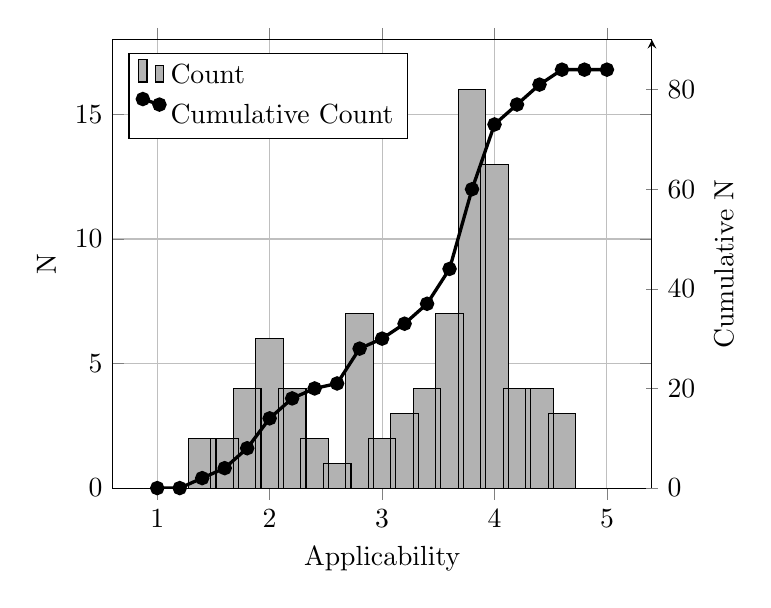
\begin{tikzpicture}
	\begin{axis} [
		xlabel=Applicability,
		ylabel=N,
		grid=major,
		legend pos=north west,
		legend cell align=left,
		ybar,
		ymin=0,
		ymax=18
	]
		\addplot[fill=black!30] coordinates {
			(1.0, 0) (1.2, 0) (1.4, 2) (1.6, 2) (1.8, 4) (2.0, 6) (2.2, 4) (2.4, 2) (2.6, 1) (2.8, 7) (3.0, 2) (3.2, 3) (3.4, 4) (3.6, 7) (3.8,16) (4.0,13) (4.2, 4) (4.4, 4) (4.6, 3) (4.8, 0) (5.0, 0)
		};
		\addlegendentry{Count}
		\addlegendimage{sharp plot,mark=*,very thick}
		\addlegendentry{Cumulative Count}
	\end{axis}
	
	\begin{axis} [
		ylabel=Cumulative N,
		axis y line=right,
		axis x line=none,
		ybar,
		ymin=0,
		ymax=90
	]
		\addplot[sharp plot,mark=*,very thick] coordinates {
			(1.0,0) (1.2,0) (1.4,2) (1.6,4) (1.8,8) (2.0,14) (2.2,18) (2.4,20) (2.6,21) (2.8,28) (3.0,30) (3.2,33) (3.4,37) (3.6,44) (3.8,60) (4.0,73) (4.2,77) (4.4,81) (4.6,84) (4.8,84) (5.0,84)
		};
	\end{axis}
\end{tikzpicture}
	\caption{Count and cumulative count of heuristics based on applicability rating by usability experts}
	\label{img:first_cumulative}
\end{figure}

Figure ~\ref{img:first_by_source} shows the percentage of heuristics achieving a given applicability rating by source. Clearly, \citeauthor{Nielsen1994a}'s heuristics performed well, as they all achieved a rating of 3.8 or more. The ratings for the heuristics developed by \citet{Singh2009} are more dispersed, but with the exception of one outlier, achieved ratings of 2.8 or more. The e-learning heuristics developed by \citet{Ardito2006} were rated least applicable to web-based CRM systems on average, but were also the most dispersed.

\begin{figure}[htbp]
	\centering
	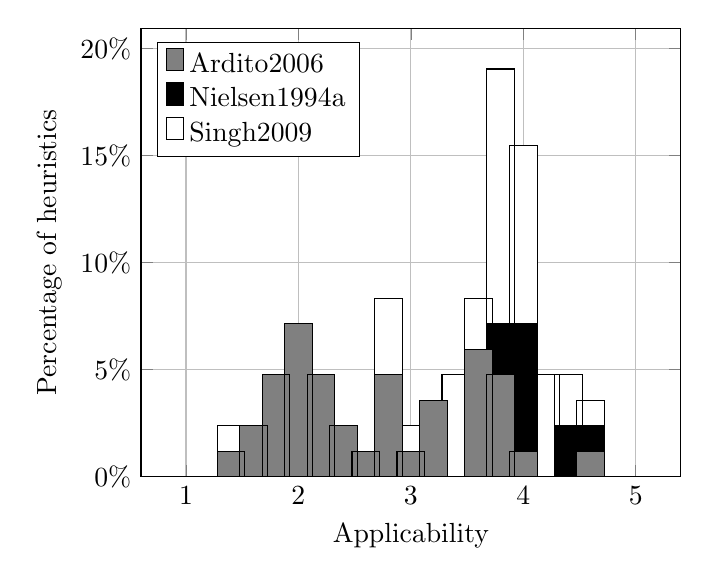
\begin{tikzpicture}
	\begin{axis} [
		xlabel=Applicability,
		ylabel=Percentage of heuristics,
		grid=major,
		legend pos=north west,
		legend cell align=left,
		ybar stacked,
		ymin=0,
		yticklabel=\pgfmathprintnumber{\tick}\%
	]
		\addplot[fill=black!50] coordinates {
			(1.00,0.00) (1.20,0.00) (1.40,1.19) (1.60,2.38) (1.80,4.76) (2.00,7.14) (2.20,4.76) (2.40,2.38) (2.60,1.19) (2.80,4.76) (3.00,1.19) (3.20,3.57) (3.40,0.00) (3.60,5.95) (3.80,4.76) (4.00,1.19) (4.20,0.00) (4.40,0.00) (4.60,1.19) (4.80,0.00) (5.00,0.00) 
		};
		\addlegendentry{\citet{Ardito2006}}
		
		\addplot[fill=black] coordinates {
			(1.00,0.00) (1.20,0.00) (1.40,0.00) (1.60,0.00) (1.80,0.00) (2.00,0.00) (2.20,0.00) (2.40,0.00) (2.60,0.00) (2.80,0.00) (3.00,0.00) (3.20,0.00) (3.40,0.00) (3.60,0.00) (3.80,2.38) (4.00,5.95) (4.20,0.00) (4.40,2.38) (4.60,1.19) (4.80,0.00) (5.00,0.00)
		};
		\addlegendentry{\citet{Nielsen1994a}}
		
		\addplot[fill=white] coordinates {
			(1.00,0.00) (1.20,0.00) (1.40,1.19) (1.60,0.00) (1.80,0.00) (2.00,0.00) (2.20,0.00) (2.40,0.00) (2.60,0.00) (2.80,3.57) (3.00,1.19) (3.20,0.00) (3.40,4.76) (3.60,2.38) (3.80,11.90) (4.00,8.33) (4.20,4.76) (4.40,2.38) (4.60,1.19) (4.80,0.00) (5.00,0.00)
		};
		\addlegendentry{\citet{Singh2009}}
	\end{axis}
\end{tikzpicture}
	\caption{Percent of all heuristics with a given rating of applicability by source}
	\label{img:first_by_source}
\end{figure}

If an applicability rating of 3 is chosen as a cut-off for selecting heuristics deemed applicable to web-based CRM systems, a total of 56 heuristics are included and 28 excluded. Of the included heuristics, 15 were developed by \citet{Ardito2006}, 10 were developed by \citet{Nielsen1994a}, and 31 were developed by \citet{Singh2009}. Table~\ref{tab:first_results_cut-off} shows the number of heuristics included from each source given an applicability rating cut-off of 3.

\begin{table}[htbp]
	\centering
	\vspace{0.5cm}
	\caption{Heuristics above and below cut-off by source}
	\label{tab:first_results_cut-off}
	\begin{tabular}{lrrrr}	\toprule
		\textbf{Source} & $\mathbf{N}$ & $\mathbf{N \boldsymbol{\geq} 3}$ & $\mathbf{N \boldsymbol{<} 3}$ & $\mathbf{\boldsymbol{\%} N \boldsymbol{\geq} 3}$ \\ \midrule
		\citet{Ardito2006} 		& 39 & 15 & 24 	&  38.64 \\
		\citet{Nielsen1994a} 	& 10 & 10 & 0 	& 100.00 \\
		\citet{Singh2009} 		& 35 & 31 & 4 	&  88.57 \\ \midrule
		Total					& 84 & 56 & 28 	&  66.67 \\
		\bottomrule
	\end{tabular}
\end{table}

A detailed table with the mean and standard deviation for each heuristic's applicability to CRM systems and need for rewording is available in appendix section~\ref{appsec:results_first}.

\FloatBarrier
\subsection{Development of New Heuristics}
The first step in developing new heuristics for web-based CRM systems was an evaluation of the heuristics with a rated need for rewording of 0.5 or more (i.e.\ more than half of the participants indicated that the heuristic needed to be reworded). All heuristics with a rating for ``need for rewording'' of 0.5 or greater were included in this activity, regardless of their applicability rating. There were a total of 13 heuristics in this category. Of the 13 heuristics, only four received a rating of applicability of three or greater. Heuristics with a low applicability rating were included, because it was anticipated their applicability could be improved through rewording.

None of the heuristics developed by \citet{Nielsen1994a} received a rating of 0.5 or greater, but six of the heuristics developed by \citet{Singh2009} and seven of the heuristics developed by \citet{Ardito2006} were in need of rewording.

The participants engaged in a group discussion focused on identifying specific problems with the heuristics in need of rewording, and establishing alternative heuristics on their basis. During the discussion, the participants identified different themes of problems with the heuristics. Table~\ref{tab:first_results_rewording_themes} gives an overview over these themes and how often they occurred. Some heuristics were associated with more than one theme.

\begin{table}[htbp]
	\centering
	\vspace{0.5cm}
	\caption[Problems identified with heuristics in need of rewording]{Problems identified with heuristics in need of rewording; A = number of heuristics per problem theme developed by \citet{Ardito2006}, S = number of heuristics per problem theme developed by \citet{Singh2009}}
	\label{tab:first_results_rewording_themes}
	\begin{tabular}{lrrrr}	\toprule
		\textbf{Problem Theme} 	& \textbf{A} & \textbf{S} & \textbf{Total} & \textbf{Reworded} \\ \midrule
		Difficult to understand & 4 & 2 & 6 & 3 \\
		Domain-specific wording & 5 & 0 & 5 & 3 \\
		Too vague and general 	& 0 & 3 & 3 & 1 \\
		Not a real heuristic	& 1 & 1 & 2 & 1 \\
		Subjective				& 0 & 2 & 2 & 1 \\
		Incomplete				& 0 & 1 & 1 & 1 \\
		Multiple meanings		& 0 & 1 & 1 & 0 \\
		\bottomrule
	\end{tabular}
\end{table}

The two most common themes were ``difficult to understand'' and ``domain-specific wording''. Of the six heuristics which were difficult to understand, two came from \citet{Singh2009} and four came from \citet{Ardito2006}. All five of the heuristics with domain-specific wording that needed to be changed were developed by \citet{Ardito2006}.

The participants were able to modify these heuristics in eight cases to create new heuristics which are more relevant to web-based CRM systems. Table~\ref{tab:first_results_rewording_themes} also shows how many of the heuristics with a certain problem theme were reworded by the participants.

There were two heuristics which received an applicability rating of three or greater, but which the usability experts were unable to reword. The first heuristic is ``Functionality to search for information that is available''. The second heuristic is ``The visual layout is well designed''. Both of them were developed by \citet{Singh2009} and the usability experts commented that they were too vague and general to be useful. In addition, the second heuristic was classified as ``subjective''.

Table~\ref{tab:first_reworded} shows a comparison between the old heuristics and the new versions. Note that in one case, the participants created two new heuristics to replace one old one, for a total of nine new heuristics.

\begin{table}[htbp]
	\centering
	\vspace{0.5cm}
	\caption[Old and new heuristics developed in first session]{Old and new heuristics developed in first session; A = heuristic developed by \citet{Ardito2006}, S = heuristic developed by \citet{Singh2009}}
	\label{tab:first_reworded}
	\begin{tabularx}{\textwidth}{XcX}	\toprule
		\textbf{Old Heuristic} & \textbf{Source} & \textbf{New Heuristic} \\ \midrule
		Clearly visualize course structure & A & Clearly visualize user workflow \\
		& & Clearly visualize employee performance \\
		Provide adaptation of the graphical aspect to the context of use & A & The system is customizable at the user level \\
		Highlight cross-references by state and course maps to facilitate topic links & A & Highlight cross-references between different types of data (e.g.\ customer issues, sales support, and marketing campaigns) \\
		Insert easy to use platform tools & A & The system conforms to platform conventions \\
		Provide communication mech\-an\-is\-ms to both students and lecturers & A & The system's communication me\-ch\-an\-isms match the needs of the users \\
		There is a correlation between the searched item and the required information & S & The results returned by a search a\-r\-e relevant to the information required by the user \\
		The output is easy to understand and interpret, whether the output is structured & S & The output style fits the type of data being displayed \\
		The system is intimidating and co\-mplex to learn and use & S & The system reduces intimidation and complexity by providing positive feedback and reinforcement, a clear path to execution, and a terminology that matches the users' language \\
		\bottomrule
	\end{tabularx}
\end{table}

In total, 63 of the existing heuristics are included and 22 are dropped. Table~\ref{tab:first_inclusion_matrix} gives an overview over the criteria for inclusion of existing heuristics as well as the number of heuristics in each group. Inclusion in the usability experts' list is based on the heuristic's rating of applicability as well as their need for rewording. All heuristics which scored an applicability rating of three or greater are included. Heuristics with an applicability rating of less than three were only included, if they received a rating of 0.5 for their need to be reworded and the participants were able to reword them.

\begin{table}[htbp]
	\centering
	\vspace{0.5cm}
	\caption[Decision matrix for inclusion or exclusion of existing heuristics]{Decision matrix for inclusion or exclusion of existing heuristics; Y = heuristic is included, N = heuristic is not included; numbers in parentheses represent the number of heuristics fulfilling the criteria; * one heuristic in this category was reworded and split into two new heuristics}
	\label{tab:first_inclusion_matrix}
	\begin{tabular}{ccccc}	\toprule
		& & \multicolumn{3}{c}{\textbf{Needs Rewording}} \\ \cmidrule(l){3-5}
		& & $\mathbf{\boldsymbol{<}0.5}$ & \multicolumn{2}{c}{$\mathbf{\boldsymbol{>}0.5}$} \\ \cmidrule(l){4-5}
		& & & \textbf{Reworded} & \textbf{Not Reworded} \\ \midrule
		\multirow{2}{*}{\textbf{Applicability}} & $\mathbf{\boldsymbol{\geq}3}$ & Y (52) & Y (2) & Y (2) \\
		& $\mathbf{\boldsymbol{<}3}$ 	& N (19) & Y ($6+1$*) & N (3) \\
		\bottomrule
	\end{tabular}
\end{table}

Of the 13 heuristics rated to be in need of rewording, four received an applicability rating of three or greater and are included in the usability experts' list of heuristics for web-based CRM systems (two of these were also reworded and the new version is included in the list). In addition, seven reworded heuristics are added to the list. These heuristics are based on existing heuristics which received an applicability rating of less than three, but have been reworded to reflect the characteristics of web-based CRM systems. Three heuristics received an applicability rating of less than three and the participants were not able to improve them by rewording, which means they are not included. Table~\ref{tab:excluded} shows the heuristics that were excluded  as well as their source and category.

\begin{table}[htbp]
	\centering
	\caption{Heuristics excluded based on criteria mentioned previously}
	\label{tab:excluded}
	\begin{tabularx}{\textwidth}{Xcc}	\toprule
		\textbf{Heuristic} & \textbf{Source} & \textbf{Category} \\ \midrule
		The capability of the system to support customization for the user at a transaction level & S & Customization \\
		The system supports alternative navigation metaphors & S & Navigation \\
		The system supports guidance-type information & S & Navigation \\
		Insert assessment tests in various forms & A & Application Proactivity \\
		Automatically update students' progress tracking & A & Application Proactivity \\
		Insert learning domain tools & A & Application Proactivity \\
		Allow different repository modes for lecturers and students & A & Application Proactivity \\
		Provide support for the preparation of the multimedia material & A & Hypermediality \\
		Maximize personalized access to learning contents & A & Hypermediality \\
		Allow repository access to both lecturer and student & A & Hypermediality \\
		Create contextualized bookmarks & A & Hypermediality \\
		Enable off-line use of platform maintaining tools and learning context & A & Hypermediality \\
		Provide the possibility to personalize interface graphics & A & Presentation \\
		Enable to define a clear learning path & A & User Activity \\
		Allow to define alternative learning paths & A & User Activity \\
		Provide support for assessment test & A & User Activity \\
		Manage reports about attendance and usage of a course & A & User Activity \\
		Allow use of learning tools even when not scheduled & A & User Activity \\
		Allow the possibility to personalize the learning path & A & User Activity \\
		Provide mechanisms to integrate the didactic material & A & User Activity \\
		Allow the possibility to create standard-com\-pliant documents and tests (AICC, IMS, SC\-O\-R\-M) & A & User Activity \\
		Provide authoring tools to facilitate documents updating and assessment tests editing & A & User Activity \\
		\bottomrule
	\end{tabularx}
\end{table}

When examining the sources of the heuristics which were dropped, it becomes quite evident, that some categories are much more prominent in the list than others. Table~\ref{tab:source_dropped_heuristics} shows the percentage of heuristics dropped from each original category. There were three categories from which more than one third of the heuristics were dropped. These categories are \textit{hypermediality} (71.4\%), \textit{user activity} (64.3\%), and \textit{application proactivity} (40\%). All three of these categories stem from the set of e-learning heuristics developed by \citet{Ardito2006}. These heuristics use domain-specific wording or make reference to domain-specific user interface elements (such as assessment tests and learning paths).

\begin{table}[htbp]
	\centering
	\caption{Categories from which heuristics were dropped with percentage of heuristics dropped}
	\label{tab:source_dropped_heuristics}
	\begin{tabular}{lcccc}	\toprule
		\textbf{Category} & \textbf{Source} & \textbf{Original \#} & \textbf{\# Dropped} & \textbf{\% Dropped} \\ \midrule
		Customization 			& S &  6 & 1 & 16.7 \\
		Navigation				& S & 10 & 2 & 20.0 \\
		Application Proactivity	& A & 10 & 4 & 40.0 \\
		Hypermediality			& A &  7 & 5 & 71.4 \\
		Presentation				& A &  8 & 1 & 12.5 \\
		User Activity			& A & 14 & 9 & 64.3 \\
		\bottomrule
	\end{tabular}
\end{table}

The second and last step in developing new heuristics was an open group discussion in which the participants were asked to identify heuristics which have not been addressed by the heuristics they saw in the previous activity. During this discussion, the participants developed five new heuristics:

\begin{itemize}
	\item The system provides appropriate filters to organize data
	\item The system allows for tailoring of the interface to an individual's workflow
	\item The system displays appropriate information depending on the task at hand
	\item The system has a dashboard which shows the current status at a quick glance
	\item Help and documentation are immersed in the system, non-obtrusive, and ubiquitous
\end{itemize}

With these five new heuristics, the final experts' list of heuristics for web-based CRM systems consists of 68 heuristics. 56 of the original heuristics were included, because they received an applicability rating of three or greater. Of these, two were reworded by the usability experts to become more applicable or clear. In addition, the reworded versions of six heuristics which received an applicability rating of less than three were included (note that one of the heuristics was reworded to result in two separate heuristics for a total of seven). Finally, five new heuristics developed by the usability experts were added. Figure~\ref{img:first_final_list} shows the composition of this list.

\begin{figure}[htbp]
	\centering
	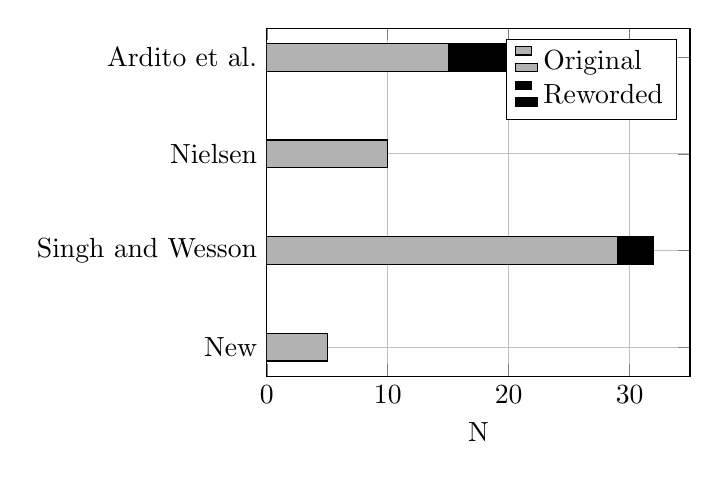
\begin{tikzpicture}
	\begin{axis} [
		height=6cm,
		xlabel=N,
		grid=major,
		legend pos=north east,
		legend cell align=left,
		xbar stacked,
		xmin=0,
		xmax=35,
		y dir=reverse,
		symbolic y coords={Ardito et al., Nielsen, Singh and Wesson, New},
	]
		\addplot[fill=black!30,xbar legend] coordinates {
			(15,Ardito et al.) (10,Nielsen) (29,Singh and Wesson) (5,New)
		};
		\addlegendentry{Original}
		
		\addplot[fill=black,xbar legend] coordinates {
			(6,Ardito et al.) (0,Nielsen) (3,Singh and Wesson) (0,New)
		};
		\addlegendentry{Reworded}
	\end{axis}
\end{tikzpicture}
	\caption{Sources of heuristics in usability experts' list}
	\label{img:first_final_list}
\end{figure}

\FloatBarrier
\section{Phase Two}
The second phase was administered between July 11th, 2012 and July 30th, 2012. The participants were asked to fill out an online questionnaire by rating the applicability of each of the heuristics from the first phase. The questionnaire also contained some background questions. After the participants filled out the questionnaire, the researcher called them to conduct a follow-up interview.

\subsection{Participants}
A total of six CRM users participated in this phase, although one of them could not be reached for the follow-up interview. All participants had at least two years of experience using a web-based CRM system. The mean number of years of experience was 5.67. With the exception of one participant, all use a CRM system daily. The other participant uses one two to three times per week. All but one of the participants had been using a web-based CRM system for the entirety of their years of experience with any CRM system. Table~\ref{tab:second_participants} gives on overview of the participants' experience.

\begin{table}[hbtp]
	\centering
	\vspace{0.5cm}
	\caption{Years of experience with CRM systems of the participants of the second phase}
	\begin{tabular}{lrrrrrr} \toprule
		& \multicolumn{6}{c}{\textbf{Participant}} \\
		\textbf{Years of Experience\ldots{}} & \textbf{F} & \textbf{G} & \textbf{H} & \textbf{I} & \textbf{J} & \textbf{K} \\ \midrule
		using a CRM system 				& 3 & 5 & 16 & 6 & 10 & 2 \\
		using a web-based CRM system	& 3 & 5 &  8 & 6 & 10 & 2 \\
		\bottomrule
	\end{tabular}
	\label{tab:second_participants}
\end{table}

Four of the participants used salesforce.com as their CRM system, one used a system called Bullhorn. The system the sixth participant used could not be determined.

\subsection{Evaluation of Usability Experts' Heuristics}
\label{sec:evaluation_existing_second}
The first activity in this phase, similarly to the first activity in the previous phase, consisted of a rating of the heuristics developed in the first phase based on their applicability to web-based CRM systems. The ratings were performed on a five-point scale ranging from ``not applicable'' (1) to ``highly applicable'' (5). There was an additional option of ``don't know'' for cases in which the participant was unable to understand the heuristic.

On average, it took the participants close to 52 minutes to complete the questionnaire. It should be noted that four of the participants took less than 45 minutes to complete the questionnaire, while it took the two others more than one hour.

A total of 68 heuristics was rated in this activity. Ten were taken from \citet{Nielsen1994a}, 32 from \citet{Singh2009}, 21 from \citet{Ardito2006}, and five were newly developed during the previous phase. Table~\ref{tab:second_results_bysource} shows selected descriptive statistics for the heuristics based on their source. Overall, the ratings of applicability were very similar and very high across all sources of heuristics. Appendix section~\ref{appsec:results_second} contains the detailed results of the rating activity.

\begin{table}[htbp]
	\centering
	\vspace{0.5cm}
	\caption{Overall applicability by heuristics source during second phase}
	\label{tab:second_results_bysource}
	\begin{tabular}{lrrrrrr} \toprule
			& & & \multicolumn4{c}{\textbf{Applicability}} \\
			\textbf{Source} & $\mathbf{N}$ & \textbf{\% Missing} & \textbf{Mean} & \textbf{Min.} & \textbf{Max.} & \textbf{St.\ Dev.} \\ \midrule
			\citet{Ardito2006} & 21 & 14.29 & 4.03 & 2 & 5 & 0.849 \\
			\citet{Nielsen1994a} & 10 & 10.00 & 4.08 & 1 & 5 & 0.614 \\
			\citet{Singh2009} & 32 & 4.69 & 4.33 & 2 & 5 & 0.699 \\
			New & 5 & 3.33 & 4.03 & 2 & 5 & 0.650 \\
		\bottomrule
	\end{tabular}
\end{table}

One exception is a heuristic which consistently received very low ratings by every participant. The heuristic is ``Users often choose system functions by mistake and will need a clearly marked `emergency exit' to leave the unwanted state without having to go through an extended dialogue. Support and undo and redo.'' by \citet{Nielsen1994a}. The mean rating for this heuristic was 1.83 with a standard deviation of 0.687. This is very surprising, as the usability experts rated this heuristic much higher, at 4.6 with a standard deviation of 0.894. Thus, this heuristic was one of the three which received the highest rating of applicability by the usability experts. This is by far the biggest distance between the ratings assigned by usability experts and CRM users for any one heuristic. Since the heuristic did receive very high ratings by the usability experts, it will remain in the list of accepted heuristics, until a measurement error can be eliminated as the reason for this discrepancy.

\begin{figure}[htbp]
	\centering
	\begin{tikzpicture}
	\begin{axis} [
		xlabel=Applicability,
		ylabel=N,
		grid=major,
		legend pos=north west,
		legend cell align=left,
		ybar stacked,
		bar width=13pt,
		ymin=0,
		ymax=16
	]
		\addplot[fill=white,pattern=north east lines] coordinates {
			(1, 0) (1.2, 0) (1.4, 0) (1.6, 0) (1.8, 0) (2, 0) (2.2, 0) (2.4, 0) (2.6, 0) (2.8, 0) (3, 2) (3.2, 1) (3.4, 2) (3.6, 1) (3.8, 2) (4, 2) (4.2, 3) (4.4, 3) (4.6, 3) (4.8, 2) (5, 0)
		};
		\addlegendentry{\citet{Ardito2006}}
		
		\addplot[fill=white] coordinates {
			(1, 0) (1.2, 0) (1.4, 0) (1.6, 0) (1.8, 1) (2, 0) (2.2, 0) (2.4, 0) (2.6, 0) (2.8, 0) (3, 1) (3.2, 0) (3.4, 0) (3.6, 1) (3.8, 0) (4, 0) (4.2, 0) (4.4, 3) (4.6, 1) (4.8, 2) (5, 1)
		};
		\addlegendentry{\citet{Nielsen1994a}}
		
		\addplot[fill=white,pattern=crosshatch dots] coordinates {
			(1, 0) (1.2, 0) (1.4, 0) (1.6, 0) (1.8, 0)(2, 0) (2.2, 0) (2.4, 0) (2.6, 0) (2.8, 0) (3, 1) (3.2, 0) (3.4, 1) (3.6, 3) (3.8, 3) (4, 1) (4.2, 2) (4.4, 9) (4.6, 5) (4.8, 4) (5, 3)
		};
		\addlegendentry{\citet{Singh2009}}
		
		\addplot[fill=black!50] coordinates {
			(1, 0)  (1.2, 0) (1.4, 0) (1.6, 0) (1.8, 0) (2, 0) (2.2, 0) (2.4, 0) (2.6, 0) (2.8, 0) (3, 0) (3.2, 1) (3.4, 0) (3.6, 0) (3.8, 1) (4, 0) (4.2, 2) (4.4, 0) (4.6, 0) (4.8, 1) (5, 0)
		};
		\addlegendentry{New}
		
		\addlegendimage{sharp plot,mark=*,very thick}
		\addlegendentry{Cumulative Count}
	\end{axis}
	
	\begin{axis} [
		ylabel=Cumulative N,
		axis y line=right,
		axis x line=none,
		ybar,
		ymin=0,
		ymax=80
	]
		\addplot[sharp plot,mark=*,very thick] coordinates {
			(1, 0) (1.2, 0)(1.4, 0)  (1.6, 0) (1.8, 1) (2, 1) (2.2, 1) (2.4, 1) (2.6, 1) (2.8, 1) (3, 5) (3.2, 7) (3.4, 10) (3.6, 15) (3.8, 21) (4, 24) (4.2, 31) (4.4, 46) (4.6, 55) (4.8, 64) (5, 68)
		};
	\end{axis}
\end{tikzpicture}
	\caption{Count and cumulative count of heuristics based on applicability rating by CRM users}
	\label{img:second_cumulative}
\end{figure}

As adumbrated previously, the heuristics received much more uniform ratings in this phase than in the previous phase. When removing the outlier discussed in the previous paragraph, the lowest mean rating received by any heuristic in this phase is 3.0, which indicates relatively good applicability and the heuristics receiving this rating would have been included in the list of accepted heuristics in the previous phase. Figure~\ref{img:second_cumulative} shows the number of heuristics with a given rating of applicability as well as the cumulative count.

Another interesting figure is the percentage of abstentions for each group of heuristics. \citet{Ardito2006} received the highest number of missing votes, followed by \citet{Nielsen1994a}. Table~\ref{tab:second_results_bysource} shows the number of votes missing by source. The percentage represents the total number of votes missing. For \citet{Ardito2006}, the maximum number of votes that could have been cast is 21 heuristics times six participants ($21*6=126$). Of these, 18 votes have not been cast, leading to an abstention rate of 14.29\%. One likely interpretation of these figures is that the participants did not feel comfortable making a decision about the heuristics because they either were unable to understand the heuristic or because they did not feel they have enough experience to make a judgment. This could mean that the participants found the heuristics by \citet{Ardito2006} much harder to understand than the heuristics developed by the usability experts in the previous phase of the study. This problem was also present in phase one, where the participants stated that the most common problem with the heuristics was that they were difficult to understand.

\subsection{Oral Comments}
During this phase, five follow-up phone interviews were conducted with the participants. One participant could not be reached despite numerous attempts. Although the researcher attempted to perform the phone interviews shortly after the participants completed the questionnaire, this was not always possible. Only in two cases could the participants be reached within 24 hours of them completing the questionnaire. The other three participants were interviewed between six and sixteen days after their completing the questionnaire. The interviews consisted of three parts corresponding to the three subsections below.

\subsubsection{Introductory Questions}
The first two questions asked in the interview were focused on the CRM systems the participants use to create some context and get them to open up and become comfortable sharing their opinion. These questions were ``What do you like most about your CRM system?'' and ``What do you like least about your CRM system?''.

The participants were fairly open in discussing these topics and all had something positive and negative to say about their CRM systems without needing to reflect for a long period of time. Overall usability of the CRM systems was the most commonly named positive and negative aspect. Some of the participants found their respective CRM system very easy to use and user-friendly, while others thought theirs was difficult to use and required ``a lot of clicking around'' to complete a task. The participants who use salesforce.com reported that they liked their CRM system better than the participants who used another system.

Another common theme was the advantage of web-based systems to be available from anywhere, even mobile devices. One participant pointed out that she can access the system when working from home on her own computer and another participant said he loved the fact that he can look up information on the go from his smartphone. The participants also pointed out that they like the fact that their CRM system synchronizes across different communication tools such as e-mail clients. This was particularly important to one participant, whose company requires her to log all oral communications and store all written communications in their CRM system. Another participant mentioned that the information she has about her clients is synchronized between her CRM system and her e-mail client, so she can have access to that information from both systems.

Information overload was mentioned as a negative aspect of CRM systems as experienced by the users. One participant said he sometimes felt overwhelmed by the amount of information in the system and the speed at which it gets created, even though the system does provide categorization and filtering of the information.

\subsubsection{Overall Impression}
This section of the interview served to discuss the participants' overall impression of the heuristics as well as their opinion of whether any heuristics were missing or areas of CRM systems that had not been covered. The questions asked in this part of the interview were ``What was your overall impression of the heuristics you saw in the questionnaire?'' and ``Do you think there is anything that is important to CRM systems that was not covered by the heuristics?''.

The participants' overall impressions of the heuristics were good. They said that most of the heuristics seemed applicable and made sense to them. Some of the participants did point out that a number of the heuristics were ``wordy'' and difficult for them to understand, but that they selected the corresponding option on the questionnaire in those cases. Another participant stated that he was unable to judge some of the heuristics since he only had experience using the CRM system as opposed to administering it. This was especially true for heuristics related to customization, as this is often done by an administrator.

When asked whether they thought anything was missing, none of the participants identified an area. This question may have been problematic and not effective in uncovering missing heuristics, since humans are typically bad at identifying things that are missing when asked outright. Another explanation might be that most of the participants were satisfied with their CRM systems for the most part and therefore weren't able to identify potential usability problems, since they don't encounter them.

The participants did mention aspects of CRM systems they liked or disliked but which were not included in the heuristics. These aspects are \textit{access from mobile devices for traveling salespeople} and \textit{synchronization of data across communication tools} (e.g.\ contact information is automatically transferred to the e-mail client and communications with a contact are available from within the CRM system). Based on these two aspects, two new heuristics are added:
\begin{itemize}
	\item The system is accessible and usable from mobile devices.
	\item The system allows for synchronization of its information with outside communication tools.
\end{itemize}

\subsubsection{Focused Evaluation of New Heuristics}
Finally, special emphasis was placed on discussing the five heuristics which were developed in the first phase to create an extra layer of validation. In this section of the interview, the five newly created heuristics were read to the participants one by one and they were asked if they thought each particular heuristic was important for web-based CRM systems.

There was overall agreement among all participants that all heuristics are important to web-based CRM systems. Only in one case, one participant stated he didn't think the heuristic ``Help and documentation are immersed in the system, non-obtrusive, and ubiquitous'' was important, because he usually contacts his company's technical support team when he has a question about the CRM system, instead of consulting the system documentation.

\section{Comparative Analysis}
\subsection{Evaluation of Existing Heuristics}
As part of the final analysis, the ratings assigned by the usability experts and the CRM users were compared. Overall, the ratings for most heuristics were higher as assigned by CRM users than by usability experts. On average, the increase amounted to 0.55 points. The heuristics which were reworded by the usability experts received a much higher rating than the original heuristics. On average, the ratings for the reworded heuristics increased by 1.92 points as compared to the original heuristics. Table~\ref{tab:rating_difference_bysource} shows the difference in ratings between phases by source.

\begin{table}[htbp]
	\centering
	\vspace{0.5cm}
	\caption{Comparison of rating differences between phases by source}
	\label{tab:rating_difference_bysource}
	\begin{tabular}{lccc}	\toprule
		\textbf{Source} & \textbf{Usability Experts} & \textbf{CRM Users} & \textbf{Difference} \\ \midrule
		\citet{Ardito2006} 		& 3.19 	& 4.03 &  0.84 	\\
		\citet{Nielsen1994a} 	& 4.10 	& 4.08 & -0.02 	\\
		\citet{Singh2009} 		& 3.79 	& 4.33 &  0.54 	\\
		New 					&  ---	& 4.03 &   ---	\\
		\bottomrule
	\end{tabular}
\end{table}

Of the five heuristics whose rating decreased the most between the two phases, the average decrease was 1.3 points. Three of these heuristics were developed by \citet{Nielsen1994a}. Table~\ref{tab:biggest_losers} gives an overview of these five heuristics. The five heuristics which experience the largest increase in ratings are shown in table~\ref{tab:biggest_winners_overall}. All of these heuristics are reworded versions of the original heuristics. Table~\ref{tab:biggest_winners_original} shows the five heuristics which received the highest increase in ratings when excluding the reworded heuristics.

\begin{table}[htbp]
	\centering
	\vspace{0.5cm}
	\caption{Heuristics whose applicability rating decreased by 0.8 points or more during phase two}
	\label{tab:biggest_losers}
	\begin{tabularx}{\textwidth}{Xcc}	\toprule
		\textbf{Heuristic} & \textbf{Source} & \textbf{Difference} \\ \midrule
		Users often choose system functions by mistake and will need a clearly marked `emergency exit' to leave the unwanted state without having to go through an extended dialogue. Support and undo and redo. & N & -2.77 \\
		The ability of the UI to be configured without affecting the underlying business logic of the system & S & -1.4 \\
		Accelerators -- unseen by the novice user -- may often speed up the interaction for the expert user to such an extent that the system can cater to both inexperienced and experienced users. Allow users to tailor frequent actions. & N & -0.8 \\
		Introduce mechanism to highlight errors and cues to avoid errors & A & -0.8 \\
		Dialogues should not contain information which is irrelevant or rarely needed. Every extra unit of information in a dialogue competes with the relevant units of information and diminishes their relative visibility. & N & -0.8 \\
		\bottomrule
	\end{tabularx}
\end{table}

\begin{table}[htbp]
	\centering
	\vspace{0.5cm}
	\caption{Heuristics with the largest rating increase}
	\label{tab:biggest_winners_overall}
	\begin{tabularx}{\textwidth}{Xcc}	\toprule
		\textbf{Heuristic} & \textbf{Source} & \textbf{Difference} \\ \midrule
			Clearly visualize employee performance & A & 2.83 \\
			Highlight cross-references between different types of data (e.g.\ customer issues, sales support, and marketing campaigns) & A & 2.63 \\
			Clearly visualize user workflow & A & 2.33 \\
			The system reduces intimidation and complexity by providing positive feedback and reinforcement, a clear path to execution, and a terminology that matches the users' language & S & 2.27 \\
			The system's communication mechanisms match the needs of the users & A & 2.17 \\
		\bottomrule
	\end{tabularx}
\end{table}

\begin{table}[htbp]
	\centering
	\vspace{0.5cm}
	\caption{Heuristics with the largest rating increase excluding reworded heuristics}
	\label{tab:biggest_winners_original}
	\begin{tabularx}{\textwidth}{Xcc}	\toprule
		\textbf{Heuristic} & \textbf{Source} & \textbf{Difference} \\ \midrule
			Functionality to search for information that is available & S & 1.6 \\
			The output provided provides clear visibility into the various other departments & S & 1.5 \\
			Clearly visualize progress tracking & A & 1.4 \\
			Maximize adaptation of technology to the context of use & A & 1.33 \\
			The system improves user productivity & S & 1.07 \\
		\bottomrule
	\end{tabularx}
\end{table}

\FloatBarrier
\subsection{Creation of New Heuristics}
During phase one, five new heuristics were created and then accepted by the participants in phase two.
\begin{enumerate}
	\item The system provides appropriate filters to organize data
	\item The system allows for tailoring of the interface to an individual's workflow
	\item The system displays appropriate information depending on the task at hand
	\item The system has a dashboard which shows the current status at a quick glance
	\item Help and documentation are immersed in the system, non-obtrusive, and ubiquitous	
\end{enumerate}

During phase two, two new heuristics were added.
\begin{enumerate}
	\setcounter{enumi}{5}
	\item The system is accessible and usable from mobile devices
	\item The system allows for synchronization of its information with outside communication tools
\end{enumerate}

To create a unified list of heuristics in appropriate categories, these seven heuristics can be added to the categories created by \citet{Singh2009}. Heuristics 1, 3, 4, and 7 can be sorted into the category \textit{task support}, 2 can be added to \textit{customization}, 6 belongs to \textit{presentation}, and 5 belongs to \textit{learnability}.

The ten heuristics developed by \citet{Nielsen1994a} can also be sorted into the categories developed by \citet{Singh2009} to create a single list of heuristics for web-based CRM systems. See table~\ref{tab:nielsen_to_singh} for the categorization of the heuristics.

\begin{table}[htbp]
	\centering
	\caption{Categorizing heuristics developed by \citet{Nielsen1994a} into categories developed by \citet{Singh2009}}
	\label{tab:nielsen_to_singh}
	\begin{tabularx}{\textwidth}{Xc} \toprule
		\textbf{Heuristic} & \textbf{Category} \\ \midrule
		Even though it is better if the system can be used without documentation, it may be necessary to provide help and documentation. Any such information should be easy to search, focused on the user's task, list concrete steps to be carried out, and not be too large. & Learnability \\
		Even better than good error messages is a careful design which prevents a problem from occurring in the first place. & Navigation \\
		Make object, actions, and options visible. The user should not have to remember information from one part of the dialogue to another. Instructions for use of the system should be visible or easily retrievable whenever appropriate. & Navigation \\
		Accelerators -- unseen by the novice user -- may often speed up the interaction for the expert user to such an extent that the system can cater to both inexperienced and experienced users. Allow users to tailor frequent actions. & Navigation \\
		The system should always keep users informed about what is going on, through appropriate feedback within reasonable time. & Presentation \\
		Dialogues should not contain information which is irrelevant or rarely needed. Every extra unit of information in a dialogue competes with the relevant units of information and diminishes their relative visibility. & Presentation \\
		Error messages should be expressed in plain language (no codes), precisely indicate the problem, and constructively suggest a solution. & Presentation \\
		The system should speak the users' language with words, phrases, and concepts familiar to the user, rather than system-oriented terms. Follow real-world conventions, making information appear in a natural and logical order. & Task Support \\
		Users often choose system functions by mistake and will need a clearly marked ``emergency exit'' to leave the unwanted state without having to go through an extended dialogue. Support and undo and redo. & Task Support \\
		Users should not have to wonder whether different words, situations, or actions mean the same thing. Follow platform conventions. & Task Support \\
		\bottomrule
	\end{tabularx}
\end{table}

\FloatBarrier
Most of the remaining heuristics by \citet{Ardito2006} can remain in their categories and are added to the final list of heuristics. Solely the two heuristics that were in the category \textit{hypermediality} are added to the category \textit{task support} instead, since it is a better fit for them. Finally, the list of heuristics for web-based CRM systems consists of the categories and heuristics displayed in table~\ref{tab:final_list}. There are a total of 70 heuristics in seven categories. Table~\ref{tab:final_list_composition} shows the composition of the final list.

\begin{table}[htbp]
	\centering
	\vspace{0.5cm}
	\caption[Composition of the final list of heuristics]{Composition of the final list of heuristics; N = \citet{Nielsen1994a}, S = \citet{Singh2009}, A = \citet{Ardito2006}}
	\label{tab:final_list_composition}
	\begin{tabular}{lcccc|c} \toprule
		\textbf{Category} & \textbf{N} & \textbf{S} & \textbf{A} & \textbf{New} & \textbf{Total} \\ \midrule
		Application Proactivity	&  0 &  0 &  6 & 0 &  6 \\
		Customization 			&  0 &  5 &  0 & 1 &  6 \\
		Learnability 			&  1 &  5 &  0 & 1 &  7 \\
		Navigation 				&  3 &  8 &  0 & 0 & 11 \\
		Presentation 			&  3 &  6 &  8 & 1 & 18 \\
		Task Support 			&  3 &  8 &  2 & 4 & 17 \\
		User Activity 			&  0 &  0 &  5 & 0 &  5 \\ \midrule
		\textbf{Total} 			& 10 & 32 & 21 & 7 & 70 \\
		\bottomrule
	\end{tabular}
\end{table}

\begin{singlespace}
		\tabulinesep=_1mm^1mm
	\begin{longtabu} to \textwidth {l X[1, p] c}
			\label{tab:final_list}\\
			\caption{Final, unified list of heuristics for web-based CRM systems}\\
			\toprule
			\textbf{Category} & \textbf{Heuristic} & \textbf{Source} \\
			\midrule
		\endfirsthead
			
			\textbf{Category} & \textbf{Heuristic} & \textbf{Source} \\
			\midrule
		\endhead
		
			\bottomrule
		\endlastfoot
		
		Application Proactivity & Introduce mechanisms to prevent usage errors & A \\
		Application Proactivity & Maximize adaptation of technology to the context of use & A \\
		Application Proactivity & Provide mechanisms for teaching-through-er\-rors & A \\
		Application Proactivity & Provide mechanisms to manage user's profiles & A \\
		Application Proactivity & Register the date of last modification of documents to facilitate updating & A \\
		Application Proactivity & The system conforms to platform conventions & A \\
		Customization & The ability of the system to be re-configured over a period of time & S \\
		Customization & The ability of the UI to be configured without affecting the underlying business logic of the system & S \\
		Customization & The alignment of the system to update existing business processes, and (or) to include new ones & S \\
		Customization & The capability of the system to support user-level customization & S \\
		Customization & The ease in which the system can be configured to a particular industry type & S \\
		Customization & The system allows for tailoring of the interface to an individual's workflow & New \\
		Learnability & A user can learn how to use the system without a long introduction & S \\
		Learnability & Even though it is better if the system can be used without documentation, it may be necessary to provide help and documentation. Any such information should be easy to search, focused on the user's task, list concrete steps to be carried out, and not be too large. & N \\
		Learnability & Help and documentation are immersed in the system, non-obtrusive, and ubiquitous & New \\
		Learnability & It is easy to become skillful at using the system within a short amount of time & S \\
		Learnability & The system reduces intimidation and complexity by providing positive feedback and reinforcement, a clear path to execution, and a terminology that matches the users' language & S \\
		Learnability & The various functions of the system can be identified by exploration & S \\
		Learnability & There is sufficient on-line help to support the learning process & S \\
		Navigation & Accelerators -- unseen by the novice user -- may often speed up the interaction for the expert user to such an extent that the system can cater to both inexperienced and experienced users. Allow users to tailor frequent actions. & N \\
		Navigation & Even better than good error messages is a careful design which prevents a problem from occurring in the first place. & N \\
		Navigation & Functionality can be found quickly and easily & S \\
		Navigation & Functionality to search for information that is available & S \\
		Navigation & Information can be easily accessed & S \\
		Navigation & Make object, actions, and options visible. The user should not have to remember information from one part of the dialogue to another. Instructions for use of the system should be visible or easily retrievable whenever appropriate. & N \\
		Navigation & The results returned by a search are relevant to the information required by the user & S \\
		Navigation & The system can guide the user through the correct sequence of transaction to complete a business process & S \\
		Navigation & The system is capable of supporting the different interaction styles of the various users & S \\
		Navigation & The UI supports efficient and accurate navigation of the system & S \\
		Navigation & There is clarity in terms of the next sequence of transactions of steps & S \\
		Presentation & Clearly and constantly indicate system state & A \\
		Presentation & Clearly visualize employee performance & A \\
		Presentation & Clearly visualize options and commands available & A \\
		Presentation & Clearly visualize progress tracking & A \\
		Presentation & Clearly visualize user workflow & A \\
		Presentation & Dialogues should not contain information wh\-ich is irrelevant or rarely needed. Every extra unit of information in a dialogue competes with the relevant units of information and diminishes their relative visibility. & N \\
		Presentation & Error messages should be expressed in plain language (no codes), precisely indicate the problem, and constructively suggest a solution. & N \\
		Presentation & Introduce mechanism to highlight errors and cues to avoid errors & A \\
		Presentation & Maintain UCD [user-centered design] at\-trib\-utes for interface graphical aspects & A \\
		Presentation & The information presented supports informed decision making & S \\
		Presentation & The information provided by the system is timely, accurate, complete and understandable & S \\
		Presentation & The output provided provides clear visibility into the various other departments & S \\
		Presentation & The output style fits the type of data being displayed & S \\
		Presentation & The system is accessible and usable from mobile devices & New \\
		Presentation & The system is customizable at the user level & A \\
		Presentation & The system should always keep users informed about what is going on, through appropriate feedback within reasonable time. & N \\
		Presentation & The UI [user interface] is intuitive & S \\
		Presentation & The visual layout is well designed & S \\
		Task Support & Highlight cross-references between different ty\-pes of data (e.g. customer issues, sales support, and marketing campaigns) & A \\
		Task Support & Supply different media channels for communication & A \\
		Task Support & The information provided by the system is in real-time & S \\
		Task Support & The responses from the system are quick and efficient & S \\
		Task Support & The system allows for synchronization of its information with outside communication tools & New \\
		Task Support & The system automates routine and redundant tasks & S \\
		Task Support & The system displays appropriate information depending on the task at hand & New \\
		Task Support & The system has a dashboard which provides a quick glance of the current status & New \\
		Task Support & The system improves user productivity & S \\
		Task Support & The system is easy to use & S \\
		Task Support & The system provides appropriate filters to organize data & New \\
		Task Support & The system should speak the users' language with words, phrases, and concepts familiar to the user, rather than system-oriented terms. Follow real-world conventions, making information appear in a natural and logical order. & N \\
		Task Support & The system supports efficient completion of tasks & S \\
		Task Support & The system supports improved information flow between the various organizational departments & S \\
		Task Support & The terminology used by the system is consistent with the terminology of the user & S \\
		Task Support & Users often choose system functions by mistake and will need a clearly marked "emergency exit" to leave the unwanted state without having to go through an extended dialogue. Support and undo and redo. & N \\
		Task Support & Users should not have to wonder whether different words, situations, or actions mean the same thing. Follow platform conventions. & N \\
		User Activity & Insert mechanisms to make annotations & A \\
		User Activity & Provide both synchronous and asynchronous communication tools & A \\
		User Activity & Provide easy-to-use authoring tools & A \\
		User Activity & Provide mechanisms for search by indexing, key or natural language & A \\
		User Activity & The system's communication mechanisms mat\-ch the needs of the users & A \\
	\end{longtabu}
\end{singlespace}